% !TEX program = xelatex
\documentclass[UTF8,11pt,fontset=none]{ctexart}
% Use the TeX-distributed AR PL SungtiL GB TrueType font.
% TrueType embedding avoids external Adobe-GB1 CMap rendering dependencies.
% A bare filename also works inside the editor compiler sandbox.
\setCJKmainfont[Script=Default,AutoFakeBold=2,AutoFakeSlant=0.2]{gbsn00lp.ttf}
\setCJKsansfont[Script=Default,AutoFakeBold=2]{gbsn00lp.ttf}
\setCJKmonofont[Script=Default,AutoFakeBold=2]{gbsn00lp.ttf}
\usepackage[a4paper,margin=2.4cm]{geometry}
\usepackage{amsmath,amssymb,booktabs,array,enumitem,xcolor,tikz,listings}
\usepackage[skins,breakable]{tcolorbox}
\usepackage{graphicx,needspace}
\usepackage{hyperref}
\definecolor{caramel}{HTML}{A9713C}
\definecolor{rosec}{HTML}{D8678F}
\definecolor{paper}{HTML}{FBF4EA}
\definecolor{inkc}{HTML}{3B2E24}
\hypersetup{colorlinks=true,linkcolor=caramel,urlcolor=rosec,
 pdftitle={逻辑斯谛方程与混沌：一条公式为什么会变得难以预测},pdfauthor={GPT}}
\linespread{1.06}
\setlength{\parskip}{0.2em}
\setlist{itemsep=0.15em,topsep=0.3em}
\newtcolorbox{keybox}[1][小结]{breakable,enhanced,colback=paper,colframe=caramel,
 boxrule=0.7pt,arc=1.5mm,left=3mm,right=3mm,top=2mm,bottom=2mm,
 title={\bfseries #1},coltitle=white,colbacktitle=caramel,fonttitle=\bfseries}
\newtcolorbox{warnbox}[1][注意]{enhanced,colback=rosec!6,colframe=rosec,
 boxrule=0.7pt,arc=1.5mm,left=3mm,right=3mm,top=2mm,bottom=2mm,
 title={\bfseries #1},coltitle=white,colbacktitle=rosec,fonttitle=\bfseries}
\lstset{language=Python,basicstyle=\ttfamily\footnotesize,
 keywordstyle=\color{caramel}\bfseries,commentstyle=\color{inkc!65},
 stringstyle=\color{rosec},breaklines=true,columns=fullflexible,
 keepspaces=true,showstringspaces=false,frame=single,rulecolor=\color{caramel!50},
 backgroundcolor=\color{paper},aboveskip=0.8em,belowskip=0.8em}
\title{\bfseries 逻辑斯谛方程与混沌\\[0.35em]
\large 一条公式，为什么会变得难以预测}
\author{数学建模笔记}
\date{2026 年 10 月}
\begin{document}
\maketitle\pagestyle{plain}\thispagestyle{empty}
\begin{keybox}[这篇文章想做的事]
把一个数乘上“增长能力”，再乘上“剩余空间”，不断重复，结果会怎样？
可能停在一个数附近，可能在两个数之间交替，也可能跳来跳去，像是有人在掷骰子。
但整个过程中，我们没有加入任何随机数。

这篇文章从零解释逻辑斯谛模型怎样描述增长，怎样由稳定走向周期倍增，
以及“确定性的混沌”究竟是什么意思。
还要先拆开一个常见混淆：\textbf{经典连续逻辑斯谛微分方程本身不会混沌；
能展示这条混沌路线的是离散逻辑斯谛映射。}
它们长得相像，却是不同的时间演化规则。（本文由 GPT 写作）
\end{keybox}

\section{先从一群不会无限增长的兔子说起}
若每只兔子平均贡献相同的增长，兔子越多，增长得越快。
不加限制地推下去，就是指数增长。但食物、活动空间和其他资源有限，
所以增长不能永远维持同样的势头。

用 $N(t)$ 表示时刻 $t$ 的数量，$K>0$ 表示环境承载量，
$a>0$ 表示数量很少时的增长率。一个最简单的修正是
\begin{equation}\label{eq:ode}
\frac{\mathrm dN}{\mathrm dt}=aN\left(1-\frac NK\right).
\end{equation}
不用先会微积分也能读这条式子：左边是“此刻增长得多快”；
右边的 $aN$ 表示数量越多，增长潜力越大，
而 $1-N/K$ 表示越接近资源上限，这种增长就压得越低。

当 $0<N<K$，右边为正，数量上升；当 $N>K$，右边为负，数量下降；
当 $N=K$，增长速度为零。$N=0$ 也是平衡，但这里主要研究正的初始数量。
这就是\textbf{连续时间的逻辑斯谛微分方程}，也译为 Logistic 方程。

\section{连续模型：平稳靠近承载量，不会自己乱跳}
把数量除以 $K$，令 $x=N/K$，就得到没有单位的比例：
$x=0.2$ 表示数量为承载量的两成，$x=1$ 表示达到承载量。
式 \eqref{eq:ode} 变成
\[
\frac{\mathrm dx}{\mathrm dt}=ax(1-x).
\]
它的解可以明确写出来。若初值 $x(0)=x_0>0$，则
\[
\boxed{x(t)=\frac{1}{1+(x_0^{-1}-1)e^{-at}}.}
\]
其中 $e^{-at}$ 随时间增大趋于 $0$，所以 $x(t)$ 趋于 $1$。
初值在 $0$ 与 $1$ 之间，曲线一路上升；初值大于 $1$，曲线一路下降。
它们都不需要越过平衡值，再来回试探。
\begin{center}
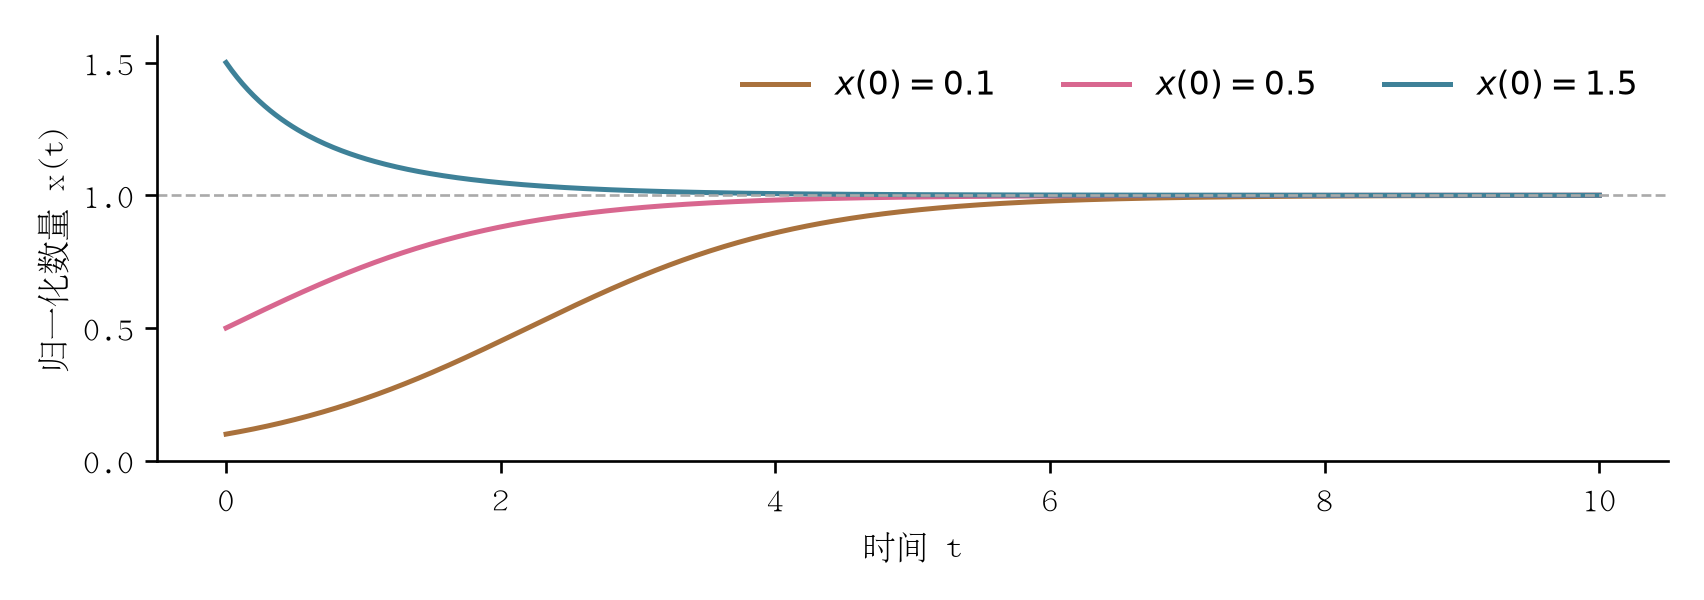
\includegraphics[width=0.86\linewidth]{images/continuous.png}

\small 取 $a=1$。三条曲线从不同初值出发，都单调靠近 $x=1$。
\end{center}
这已经说明经典模型不会产生下文那样的周期倍增和混沌。
在这种只有一个状态变量、规则不随时间变化且光滑的微分方程里，
解也不能随意越过平衡点：一旦到达平衡点，解的唯一性就要求它停在那里。
我们不需要用一张“看起来平滑”的数值图来代替这个理由。

\section{另一种规则：每过一代才更新一次}
\subsection{把“变化速度”换成“下一代的数量”}
如果研究的是一代接一代的繁殖，可以直接规定离散更新规则
\begin{equation}\label{eq:map}
\boxed{x_{n+1}=rx_n(1-x_n).}
\end{equation}
这就是\textbf{逻辑斯谛映射}：$n=0,1,2,\dots$ 表示代数，
$x_n$ 是第 $n$ 代的归一化数量，$r$ 是固定的更新参数。
“映射”在这里就是一台输入一个数、输出下一个数的机器。
连续模型中的增长率叫 $a$，离散模型中的参数叫 $r$，是为了不把二者误当成同一个量。

$rx_n$ 表示低密度时的繁殖潜力，$1-x_n$ 表示密度抑制。
这里的归一化尺度不能照搬成“种群最终一定达到的承载量”：
离散模型的正平衡值其实是 $1-1/r$，稍后会算出来。
它是一个极简的密度反馈模型，不是对所有真实种群的精确生物规律。

\subsection{为什么通常只看 \texorpdfstring{$0\le r\le4$}{0 到 4 之间的 r}}
先要求初值 $x_0\in[0,1]$。因为
\[
x(1-x)=\frac14-\left(x-\frac12\right)^2,
\]
所以 $0\le x(1-x)\le1/4$，从而
\[
0\le rx(1-x)\le r/4\le1.
\]
这样更新后仍在 $[0,1]$ 内，下一代可以接着算。
若 $r>4$，就有初值被送出这个区间，可能产生不适合数量解释的值；本文不讨论它。

\begin{warnbox}[长得像，不等于“连续方程每隔一代看一次”]
微分方程右边 $ax(1-x)$ 是\textbf{变化速度}，
映射右边 $rx(1-x)$ 是\textbf{下一步的状态}。不能把左边换一下就说它们是同一个模型。
连续方程每隔固定时长做一次精确观测，得到的更新也不是式 \eqref{eq:map}。
本文末尾会把真正的取样公式写出来。
\end{warnbox}

\section{先用计算器看一眼：同一公式，不同参数}
取 $x_0=0.2$，固定 $r$，每次把刚得到的结果放回右边，就是\textbf{迭代}。
例如 $r=2.5$ 时，前几步为
\[
0.2\ \longrightarrow\ 0.4\ \longrightarrow\ 0.6\ \longrightarrow\ 0.6\ \longrightarrow\cdots.
\]
这组数恰好第二次更新后停在 $0.6$，其他初值一般是逐渐靠近它。
若 $r=3.2$，开头则为
\[
0.2\ \longrightarrow\ 0.512\ \longrightarrow\ 0.7995392\ \longrightarrow\ 0.512884\cdots.
\]
继续计算，会在约 $0.513045$ 和 $0.799455$ 两个值附近交替。
\begin{center}
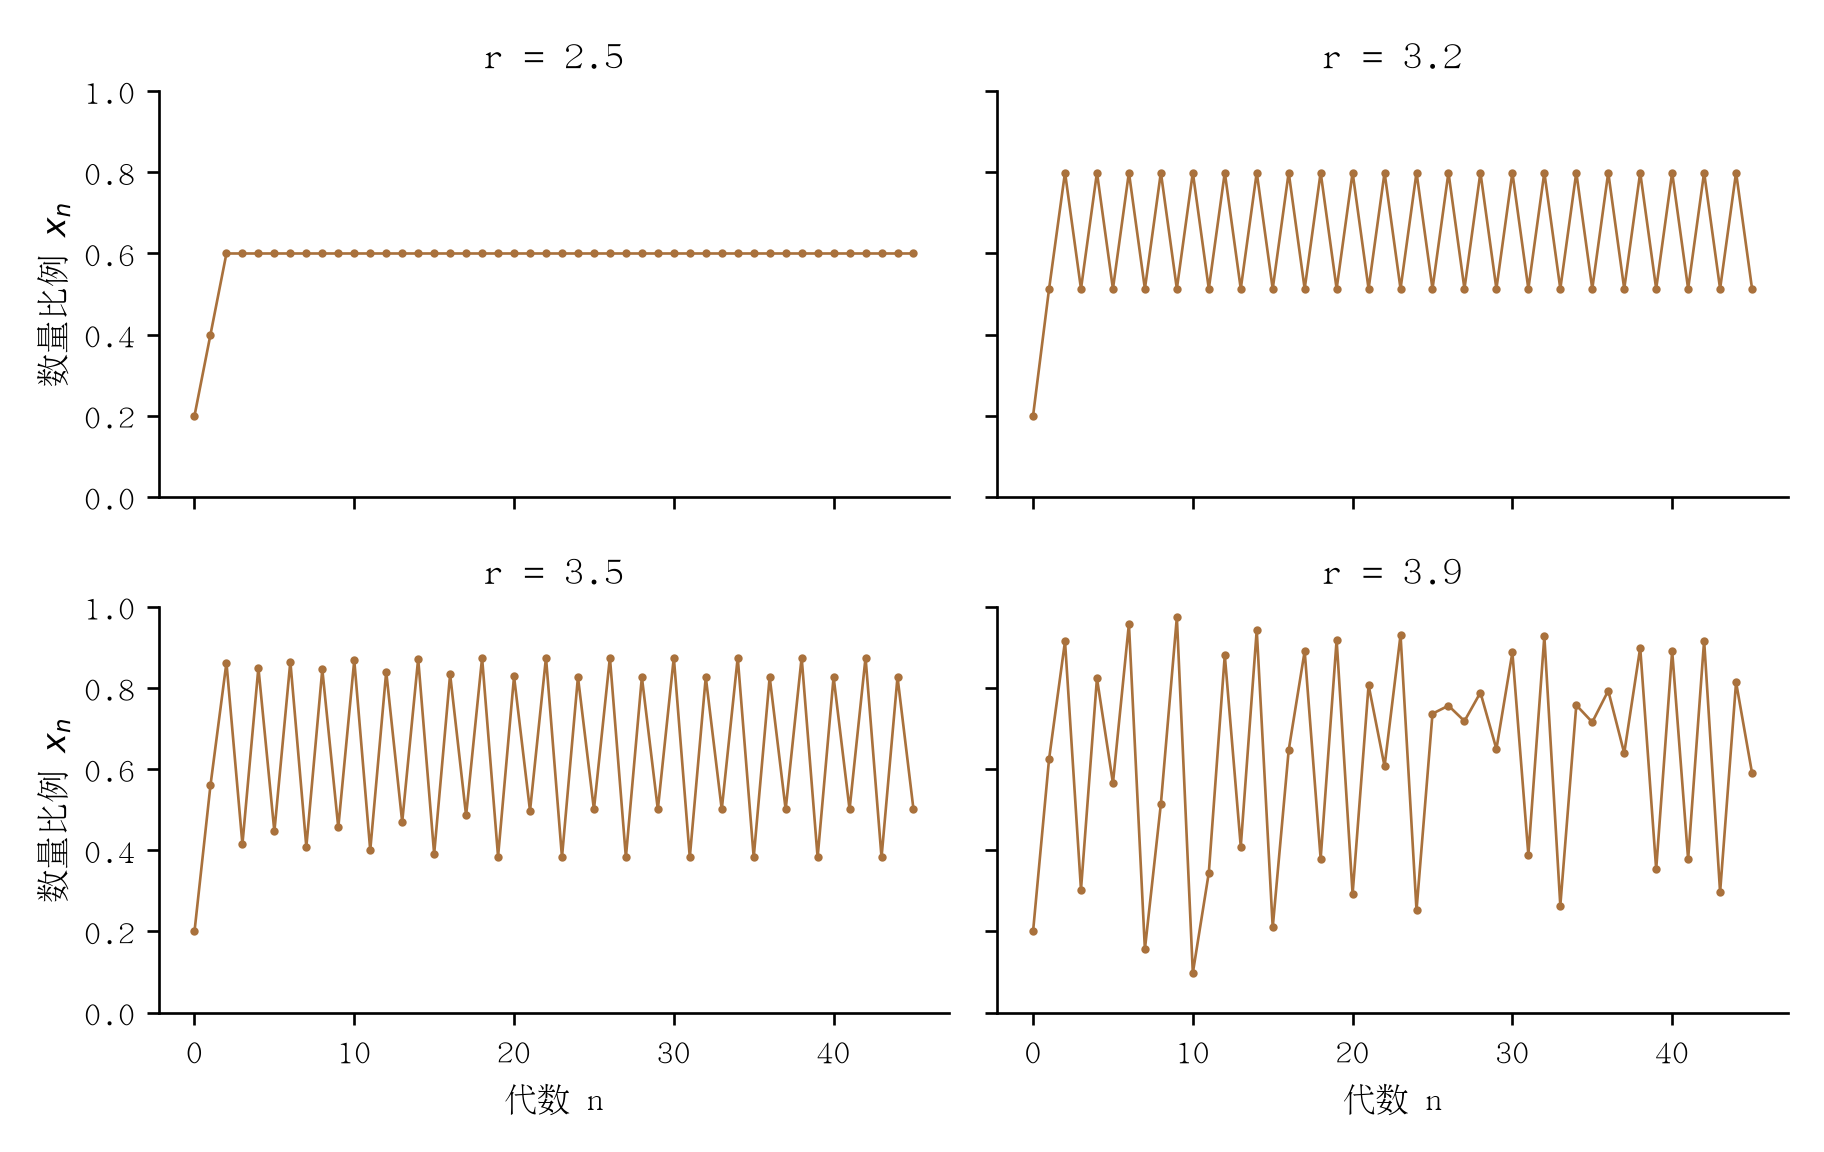
\includegraphics[width=0.9\linewidth]{images/iterations.png}

\small 同取 $x_0=0.2$，画出前 $45$ 次更新。线段只是帮助看顺序，模型只定义整数代上的值。
\end{center}
$r=2.5$ 时趋于一个值；$r=3.2$ 时趋于两个值；$r=3.5$ 时趋于四个值；
$r=3.9$ 时在这段观测里不呈现短周期。
最后一句只是图像观察，\textbf{一条不规则折线本身还不能证明混沌}。

\section{为什么有的数能把附近的轨道吸过来}
\subsection{不动点：放进去，还是它自己}
若某个 $x_*$ 满足 $x_*=rx_*(1-x_*)$，它就叫\textbf{不动点}。
解这个方程，得到
\[
x_*=0,\qquad x_*=1-\frac1r\quad(r>0).
\]
第二个点在 $r>1$ 时位于区间内部。比如 $r=2.5$ 时，它就是 $0.6$。

但“自己能停住”与“旁边的点也会靠过来”不同。
把稍微偏离它的初值记为 $x_*+\varepsilon$，其中 $\varepsilon$ 是很小的偏差。
对 $f(x)=rx(1-x)$，直接展开就有
\[
f(x_*+\varepsilon)-f(x_*)
=r(1-2x_*)\varepsilon-r\varepsilon^2.
\]
偏差足够小时，平方项比一次项小得多，所以下一步偏差近似为
\[
\varepsilon_{n+1}\approx r(1-2x_*)\varepsilon_n.
\]
我们甚至不必先学习导数，也能看出关键是\textbf{偏差每次被乘了多少}。
用导数的记法，这个倍数就是 $f'(x_*)$，其中 $f'(x)=r(1-2x)$。

\begin{keybox}[稳定性的读法]
乘数的绝对值小于 $1$，附近偏差会缩小，不动点是\textbf{局部吸引的}；
绝对值大于 $1$，附近偏差会放大，不动点不稳定。
负号表示偏差换边：本轮在平衡值上方，下轮可能跑到下方。
若绝对值恰好等于 $1$，这项近似不足以判断，要再看更高阶项。
\end{keybox}
在 $x_*=0$ 处，乘数为 $r$；因此 $0<r<1$ 时，小数量逐步衰减到零。
在正不动点处，乘数为
\[
r\left(1-2\left(1-\frac1r\right)\right)=2-r.
\]
所以它局部吸引的参数区间是
\[
|2-r|<1\quad\Longleftrightarrow\quad1<r<3.
\]
这里没有把 $r=1$ 或 $r=3$ 的边界情形硬塞进一阶判断。
对典型的区间内部初值，这个稳定区间也解释了前面看到的单点收敛。

\section{不动点失稳以后：两个值、四个值、八个值}
当 $r$ 从 $3$ 的左侧穿过 $3$，正不动点的乘数穿过 $-1$。
“左右来回但越来越近”变成“左右来回却不再缩小”，并出现一个吸引的两周期轨道。

\textbf{周期为 $2$}，是说两个不同的数 $p,q$ 满足
\[
f(p)=q,\qquad f(q)=p.
\]
走一步换到另一个，走两步回到原处。两周期的两个值可算为
\[
p,q=\frac{r+1\mp\sqrt{(r-3)(r+1)}}{2r}\qquad(r>3).
\]
若暂时不想跟二次方程打交道，可以跳过这个根式，只记住“稳定的不是一个数，而是一对交替的数”。

在两周期附近，一次乘 $f'(p)$，再乘 $f'(q)$，
所以两步后的误差乘数是 $f'(p)f'(q)=4+2r-r^2$。
令其绝对值小于 $1$，得到稳定两周期区间
\[
3<r<1+\sqrt6\approx3.449490.
\]
再往后，两周期也失稳，吸引轨道的周期变成 $4$，继而 $8$、$16$……
这种结构变化叫\textbf{分岔}，这条路线叫\textbf{周期倍增}。

\begin{center}
\begin{tabular}{ll}
\toprule
参数变化的位置 & 倍增序列中的变化\\\midrule
$r=3$ & 从稳定不动点转向两周期\\
$r=1+\sqrt6\approx3.449490$ & 两周期转向四周期\\
$r\approx3.544090$ & 四周期转向八周期\\
$r\approx3.564407$ & 八周期转向十六周期\\
$r_\infty\approx3.569945672$ & 这串倍增临界值的聚点\\\bottomrule
\end{tabular}
\end{center}
表中说的是参数跨过这些位置时的变化，不是在说临界点本身都具有某个简单的吸引周期。
聚点附近的临界行为比普通稳定周期或典型混沌都更微妙。

\section{怎样读分岔图：一列点是一种长期行为}
下面这张图横轴是 $r$，纵轴是 $x$。
对每个 $r$，都从 $x_0=0.219$ 出发，先迭代 $1800$ 次不画，
再把后面 $600$ 次的值画在这一列。前面舍弃的阶段叫\textbf{过渡过程}。
\begin{center}
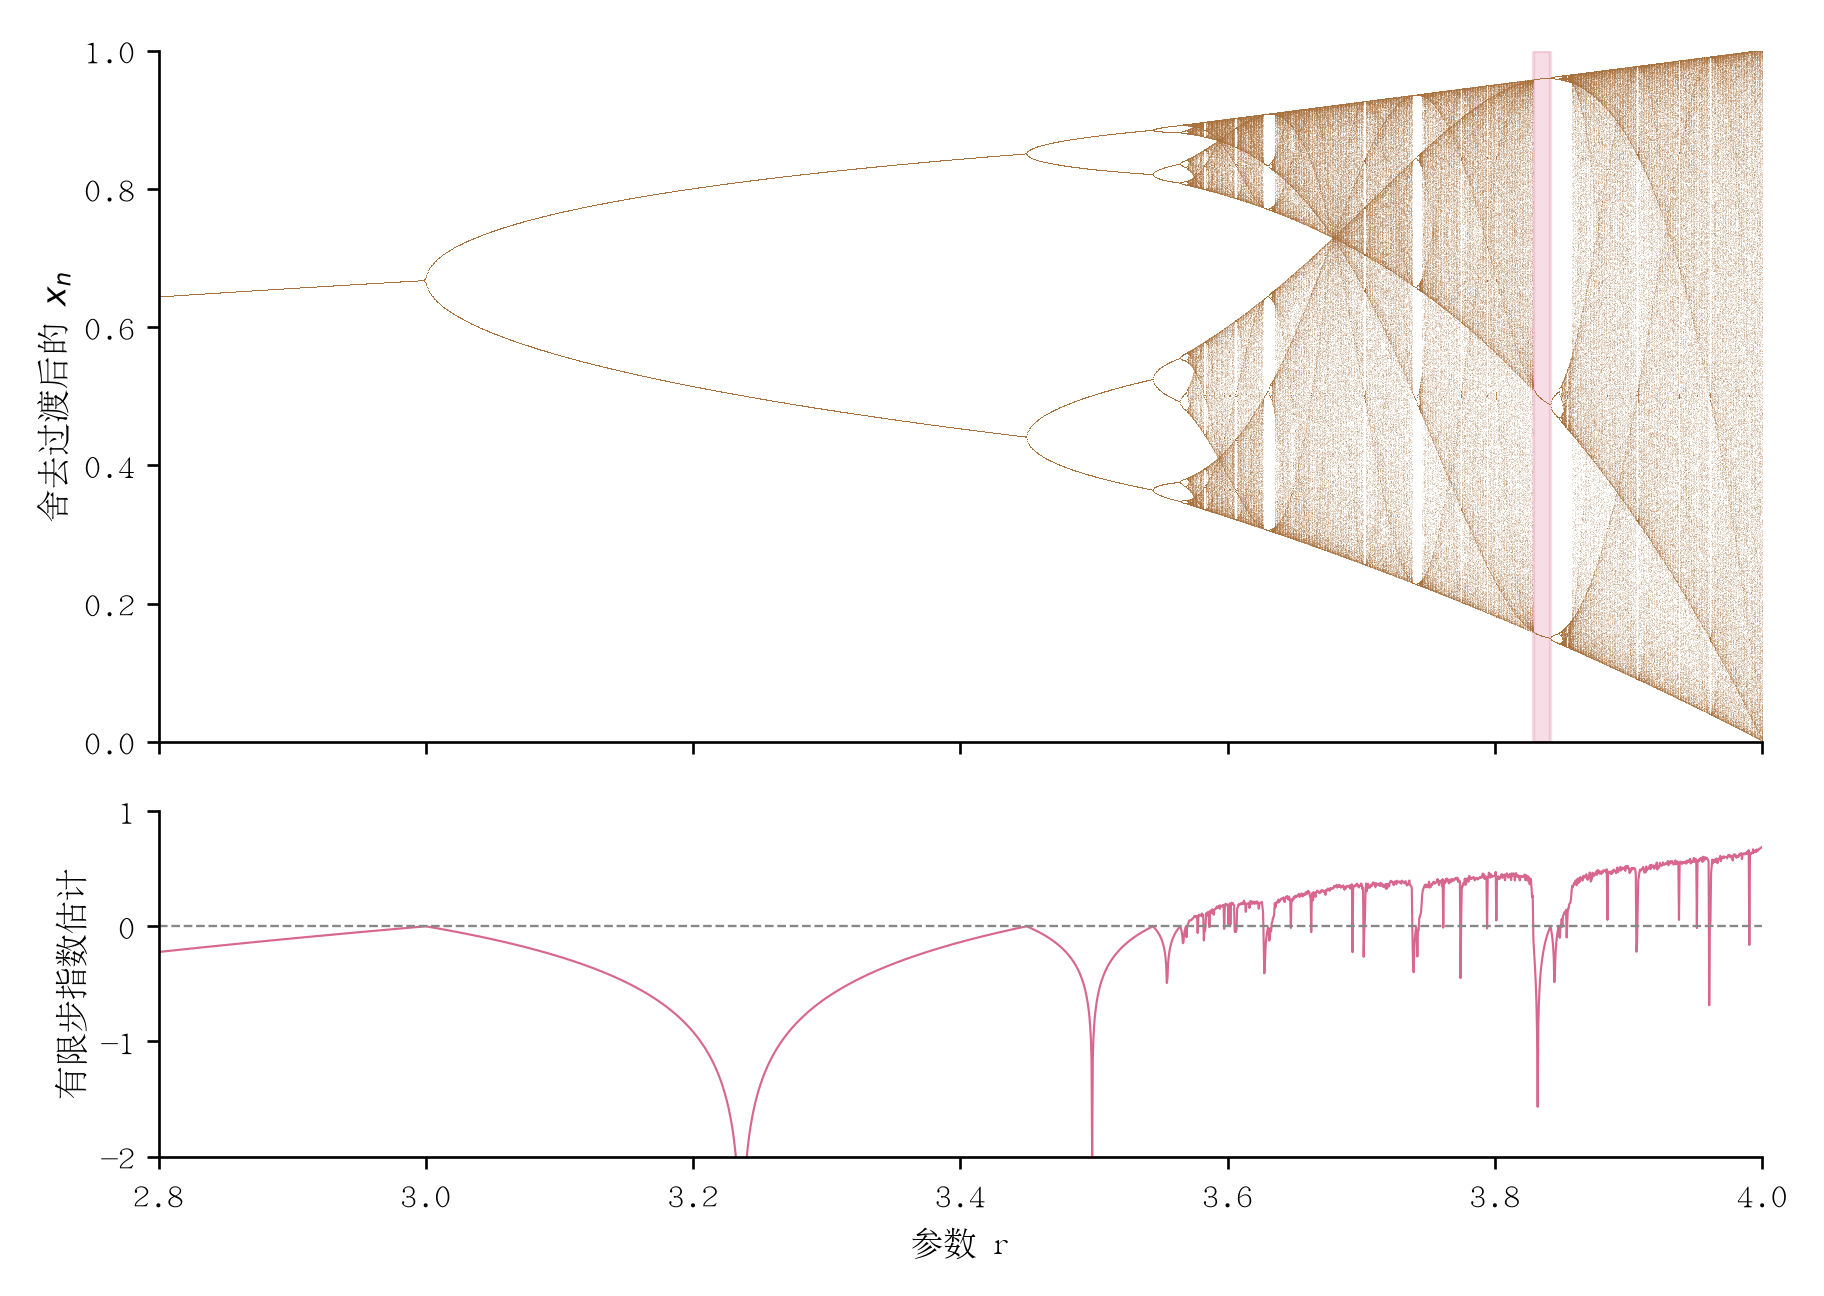
\includegraphics[width=0.94\linewidth]{images/bifurcation.png}

\small 上：分岔图。下：同一批参数上的有限步 Lyapunov 指数估计，含义见后文。
粉色竖带标出三周期窗口附近的一小段。
\end{center}
读一列：一个吸引值是一条细枝，两个交替值是上下两枝，四周期是四枝。
之后密集的点带表示在有限观测中出现了许多不同值。
读整张图：分枝不断倍增，随后又有一段段整齐的小窗口嵌在复杂区域里。

\begin{warnbox}[不是“超过 3.57，就全部混沌”]
$r_\infty$ 标出的是前面那条周期倍增级联的聚点，
不是把之后所有参数一刀切成混沌的开关。
例如 $r=3.83$，从一般初值出发会靠近稳定的三周期轨道；窗口里还可以再发生周期倍增。
有限步数、单个初值和有限像素的图，不能代替对每个参数的严格分类。
\end{warnbox}

\section{混沌的关键：规则确定，初值误差却会被放大}
设 $r=4$，分别从 $0.200000000$ 和 $0.200000001$ 开始，初始差只有十亿分之一。
前面若干步几乎看不出区别，之后两条曲线却明显分开。
这叫\textbf{对初始条件的敏感依赖}。
\begin{center}
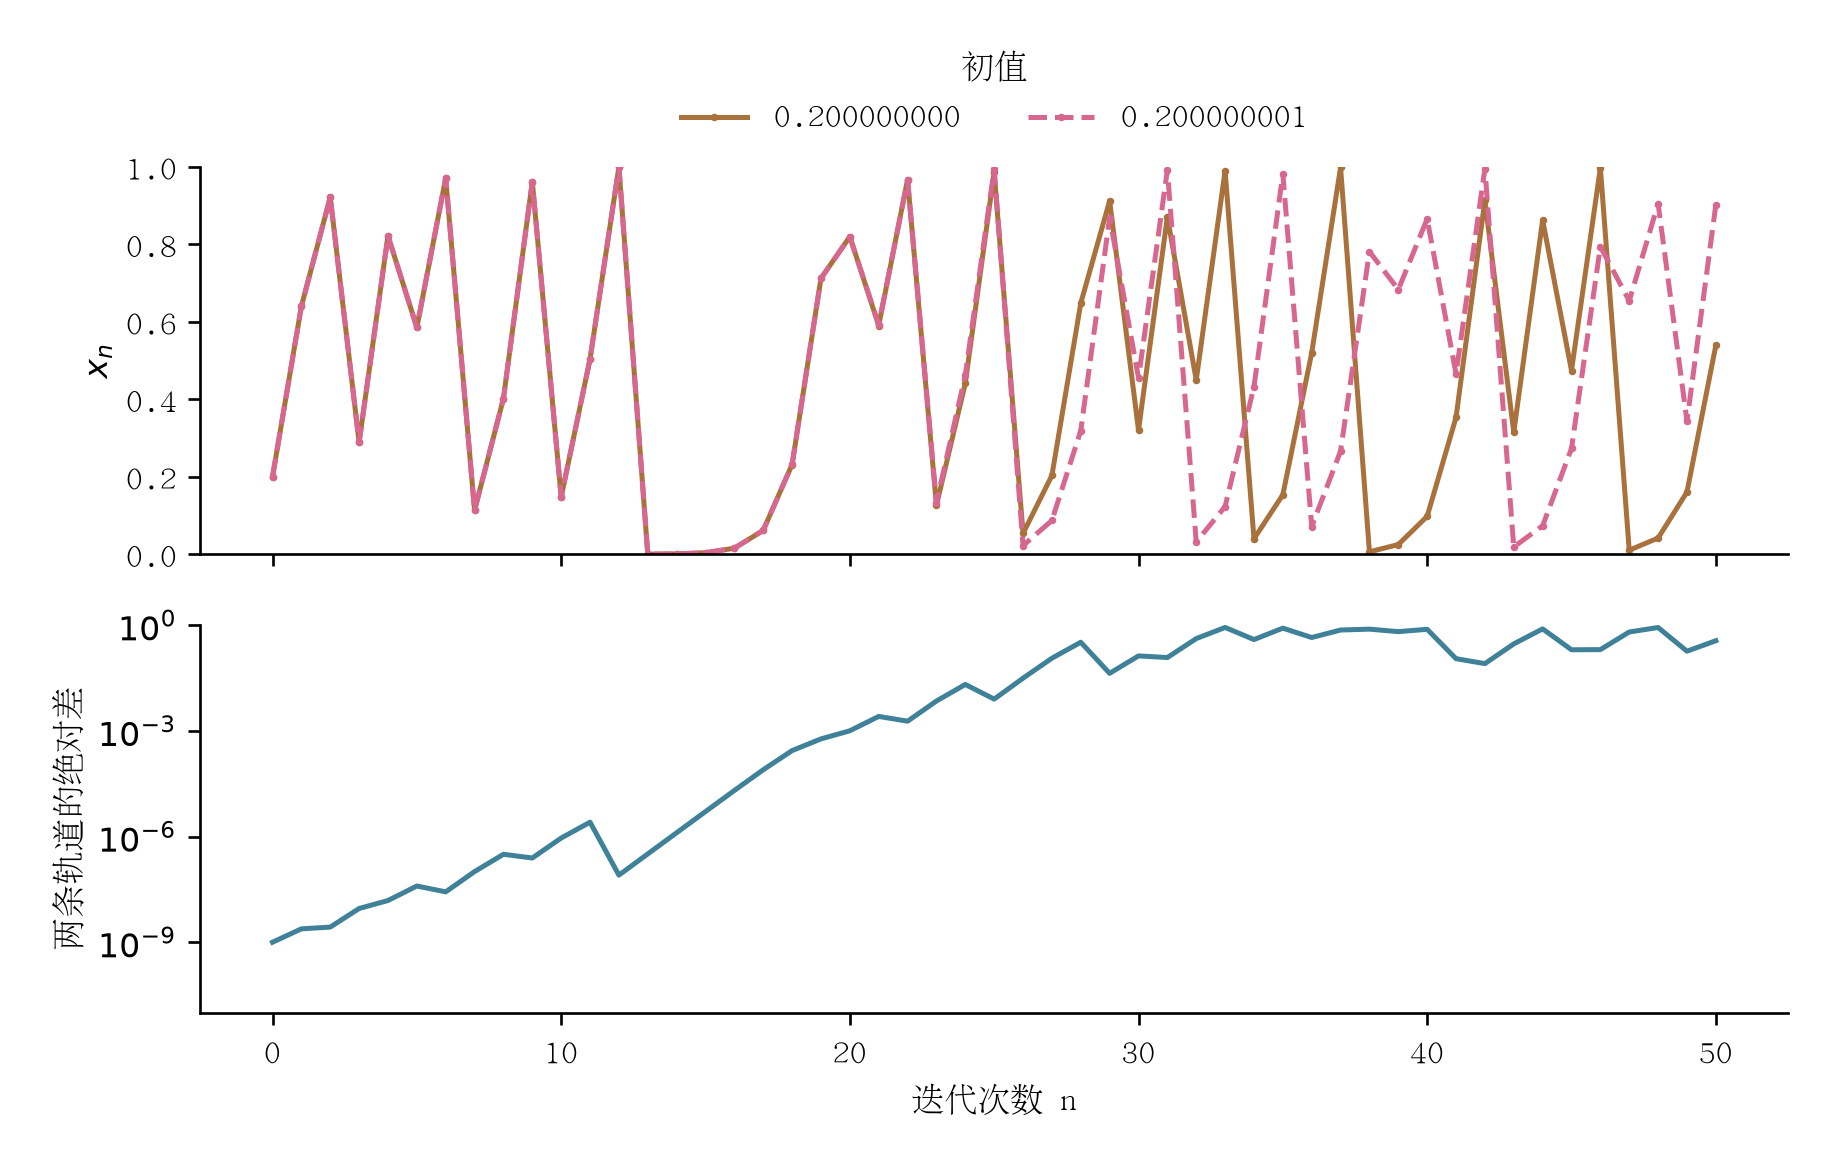
\includegraphics[width=0.9\linewidth]{images/sensitivity.png}

\small 用 $90$ 位十进制精度计算 $50$ 步。下图采用对数纵轴，以同时看清十亿分之一级与十分之一级的差值。
\end{center}
这里没有掷骰子。\textbf{完全相同的精确初值，始终产生完全相同的轨道}。
问题是现实测量通常不能提供无限精确的初值；
即使规则完全知道，有限误差也可能使远期的逐点预测失去实用意义。

这也不表示两个轨道从此永不靠近。它们被限制在 $[0,1]$ 内，会折回、穿插，
距离可以暂时变小；敏感依赖不是要求差距每一步都增大，更不是无限增大。
在本次实验中，绝对差首次超过 $0.1$ 出现在第 27 步。
这个数字依赖初值和阈值，不是一条普遍常数。

\section{伸长与折回：为什么简单的曲线装得下复杂性}
抛物线 $f(x)=4x(1-x)$ 的最高点在 $x=1/2$，两边斜率的方向相反。
在斜率绝对值大于 $1$ 的地方，邻近输入可能被拉开；
但输出始终被压回有限区间，不能一直沿同一方向逃走。

可以把它想成反复拉长并折回的一条带子：
\textbf{局部的拉伸放大细节，整体的折回让轨道留在同一个有限范围里。}
这是一幅帮助理解的几何图景，还不是“任何带弯的函数都会混沌”的定理。
$r$ 较小时，同样的抛物线就有稳定吸引点。

\Needspace{12\baselineskip}
\subsection{一个可以算出来的窗口：\texorpdfstring{$r=4$}{r=4}}
令
\[
x_n=\sin^2(\pi\theta_n).
\]
由 $4\sin^2u\cos^2u=\sin^2(2u)$，更新变成
\[
\theta_{n+1}=2\theta_n\pmod1.
\]
“$\pmod1$”表示只保留小数部分，比如 $2\times0.7=1.4$ 变成 $0.4$。
这解释了“乘二拉开，再绕回区间”的意思。

如果把 $\theta_0$ 写成二进制小数 $0.b_1b_2b_3\cdots$，
一次更新就把最前面的二进制位移走：$0.b_2b_3b_4\cdots$。
初值里很靠后的细节，会被一步步推到前面，变得重要。
$x=\sin^2(\pi\theta)$ 不是一一对应的换元，但足以把这套倍增动力学投影成 $r=4$ 的逻辑斯谛轨道。

\begin{warnbox}[混沌系统仍然有特殊轨道]
例如 $r=4$ 时，$x_0=1/2$ 会走成 $1/2\to1\to0\to0$；
$x_0=3/4$ 则一直不动。这些都是精确数学中的例子。
说“$r=4$ 具有混沌动力学”，不等于说每个初值都走出一条不重复的轨道。
\end{warnbox}

\section{怎样量化“平均会把误差放大多少”}
只看某一步的斜率不够，因为后面可能扩张，也可能收缩。
若两条轨道还足够近，经过 $N$ 步，误差近似乘上
\[
|f'(x_0)|\,|f'(x_1)|\cdots|f'(x_{N-1})|.
\]
直接相乘不方便，取自然对数就把乘法变成加法，再除以步数取平均：
\[
\boxed{\lambda=\lim_{N\to\infty}\frac1N
\sum_{n=0}^{N-1}\ln|r(1-2x_n)|.}
\]
在极限存在的轨道上，这叫\textbf{Lyapunov 指数}（李雅普诺夫指数）。
\begin{itemize}
\item $\lambda<0$：局部小偏差平均收缩，常见于稳定不动点或稳定周期轨道。
\item $\lambda>0$：无穷小偏差平均指数放大，是识别混沌的重要指标。
\item $\lambda=0$：可能处于临界情形，不能据此简单归类。
\end{itemize}
“指数放大”可以粗略写成 $\delta_n\approx\delta_0e^{\lambda n}$，
但它只描述误差尚小时的尺度。一旦误差已和区间一样大，这个近似就不能继续外推。

对 $r=4$ 的典型轨道，$\lambda=\ln2\approx0.6931$，
相当于小误差的典型增长因子约为每步 $2$。
若初始误差为 $10^{-9}$，允许误差为 $0.1$，粗略的预测时限为
\[
n\approx\frac{\ln(0.1/10^{-9})}{\ln2}\approx26.6\ \text{步}.
\]
这不是每条轨道的精确倒计时，前面的实际实验也不必恰在第 $27$ 步越过阈值。

\begin{center}
\begin{tabular}{lll}
\toprule
$r$ & 数值实验中的长期形态 & 指数估计\\\midrule
2.5 & 稳定不动点 & $-0.6931$\\
3.2 & 稳定两周期 & $-0.9163$\\
3.5 & 稳定四周期 & $-0.8725$\\
3.83 & 稳定三周期 & $-0.3698$\\
3.9 & 混沌参数的典型轨道 & $+0.4965$\\
4 & 混沌参数的典型轨道 & $+0.6931$\\\bottomrule
\end{tabular}
\end{center}
本表从 $x_0=0.219$ 出发，舍去 $2000$ 步，再平均 $20000$ 步，数字仅为有限步估计。
正指数是局部误差增长的信息，不应在任意系统里被单独当成所有混沌定义的充分条件；
例如仅仅在一个不稳定不动点上计算，也可能得到正值。

\section{回到开头：离散化会不会“制造”混沌}
对连续方程，真正每隔 $h>0$ 时间取样，精确更新为
\[
x_{n+1}=\frac{e^{ah}x_n}{1+(e^{ah}-1)x_n}.
\]
它对非负的 $x_n$ 严格递增，并且仍然把正初值单调引向 $1$。
\textbf{隔一段时间看一次，并不会把原方程变成混沌。}

但若用最简单的欧拉近似：
\[
x_{n+1}=x_n+ha\,x_n(1-x_n),
\]
这次右边多了一个原来的 $x_n$。
令 $k=ha$，再缩放 $y_n=kx_n/(1+k)$，就可化为
\[
y_{n+1}=(1+k)y_n(1-y_n).
\]
它确实具有逻辑斯谛映射的形式，参数是 $r=1+k$。
若步长取得太粗，它可能失稳，甚至出现原连续方程没有的复杂行为。
例如在 $x=1$ 附近，欧拉迭代的误差乘数为 $1-ha$，
$ha>2$ 就已经破坏了该平衡的局部稳定性。

\begin{keybox}[两种来源，要分别判断]
若离散更新本来就是所选的代际模型，就研究这个离散模型本身的动力学。
若离散更新只是为了数值近似某个连续方程，
则应减小步长、比较精确解或更可靠的数值方法，检查看到的波动是否为数值伪象。
“电脑画出来很乱”不等于“原来的物理系统必然混沌”。
\end{keybox}

\section{最后一个实验提醒：电脑并没有无限精度}
普通浮点数只有有限多个可表示状态。
同一台机器用固定的计算规则反复迭代，只要某个状态重复，后面就会整个重复，
所以最终一定进入某个机器周期，尽管可能很长。
这不能用来否定实数模型中的混沌；反过来，一段有限折线不重复也不能证明它永不重复。

本文的初值敏感性图使用高精度十进制计算，并比较了 $90$ 位与 $120$ 位精度下的前 $50$ 步，
确认这段分离不是普通浮点舍入制造的。
分岔图则仍是有限参数网格、有限迭代次数的数值展示；
在临界点附近，过渡过程可能很长，不能把“舍去 $1800$ 步”当作普遍收敛保证。

随文的 \texttt{数值实验.py} 可重新生成所有四张图，并核验不动点、两周期根式、
四周期、三周期和指数的若干已知结果。它需要 NumPy 与 Matplotlib；
图中的中文使用 TeX Live 随附的文鼎宋体，其他机器可以调整程序顶部的字体文件位置。

\begin{keybox}[这条路线到底告诉了我们什么]
\begin{enumerate}
\item 连续逻辑斯谛方程描述平滑趋稳的增长；离散逻辑斯谛映射可能出现不同动力学。
\item 参数变大时，稳定不动点可经两周期、四周期、八周期的倍增级联走向复杂行为。
\item 混沌来自确定规则本身的动力学，不需要外部随机数；初值精度有限，会限制远期逐点预测。
\item 混沌区域里仍有周期窗口，混沌参数下也有特殊周期轨道，不能只按一个阈值或一张折线判断。
\item 数值实验应和解析推理互相检查，并分清数学模型、离散近似与机器精度这三层问题。
\end{enumerate}
\end{keybox}

\begin{keybox}[参考与继续阅读]
\begin{itemize}
\item R.~M.~May，\href{https://doi.org/10.1038/261459a0}{Simple mathematical models with very complicated dynamics}，
\textit{Nature} \textbf{261}（1976），459--467。了解简单差分模型中稳定、周期与复杂动力学的经典入口。
\item B.~Deng，\href{https://www.math.unl.edu/~bdeng1/Research/Book\%20Project/PartFour.pdf}{All Systems}，
大学课程讲义，第 3 章讨论逻辑斯谛映射的周期倍增与临界参数。
\end{itemize}
\end{keybox}
\end{document}
